\newpage
\section{Korrelationsmatrizen sortiert nach der Bevölkerungsdichte}\label{sec:Durchführung:Korrelationsmatrizen sortiert nach der Bevölkerungsdichte}
In den folgenden beiden Abschnitten \autoref{sec:Durchführung:Korrelationsmatrizen mit den nach Bevölkerungsdichten sortierten Landkreisen} und \autoref{sec:Durchführung:Korrelationsmatrizen mit den nach Bevölkerungsdichten sortierten Regierungsbezirken} sind die Werte der Korrelationsanalysen als Matrizen dargestellt, wie es in \autoref{sec:BeschreibungKorrelationsanalyse} definiert und in \autoref{sec:Vorgehensweise:Korrelationsanalyse} beschrieben ist.
\subsection{Korrelationsmatrizen mit den nach Bevölkerungsdichten sortierten Landkreisen}\label{sec:Durchführung:Korrelationsmatrizen mit den nach Bevölkerungsdichten sortierten Landkreisen}
In \autoref{fig:matrizes_pop_density_counties} finden sich die vier Matrizen mit den Werten für die Korrelationen zwischen allen Landkreisen. Die Zeilen und Spalten sind nach der Bevölkerungsdichte der Landkreise sortiert. Im Anhang in \autoref{tab:counties_by_pop_density} befindet sich die vollständige Auflistung.

Bis auf eine kleine Überzahl an negativen Werten an der linken Seite und der entsprechenden Spiegelung mit negativem Vorzeichen an der ersten Winkelhalbierenden scheinen die Matrizen relativ homogen besetzt zu sein.

\begin{figure}[H]
    \centering
    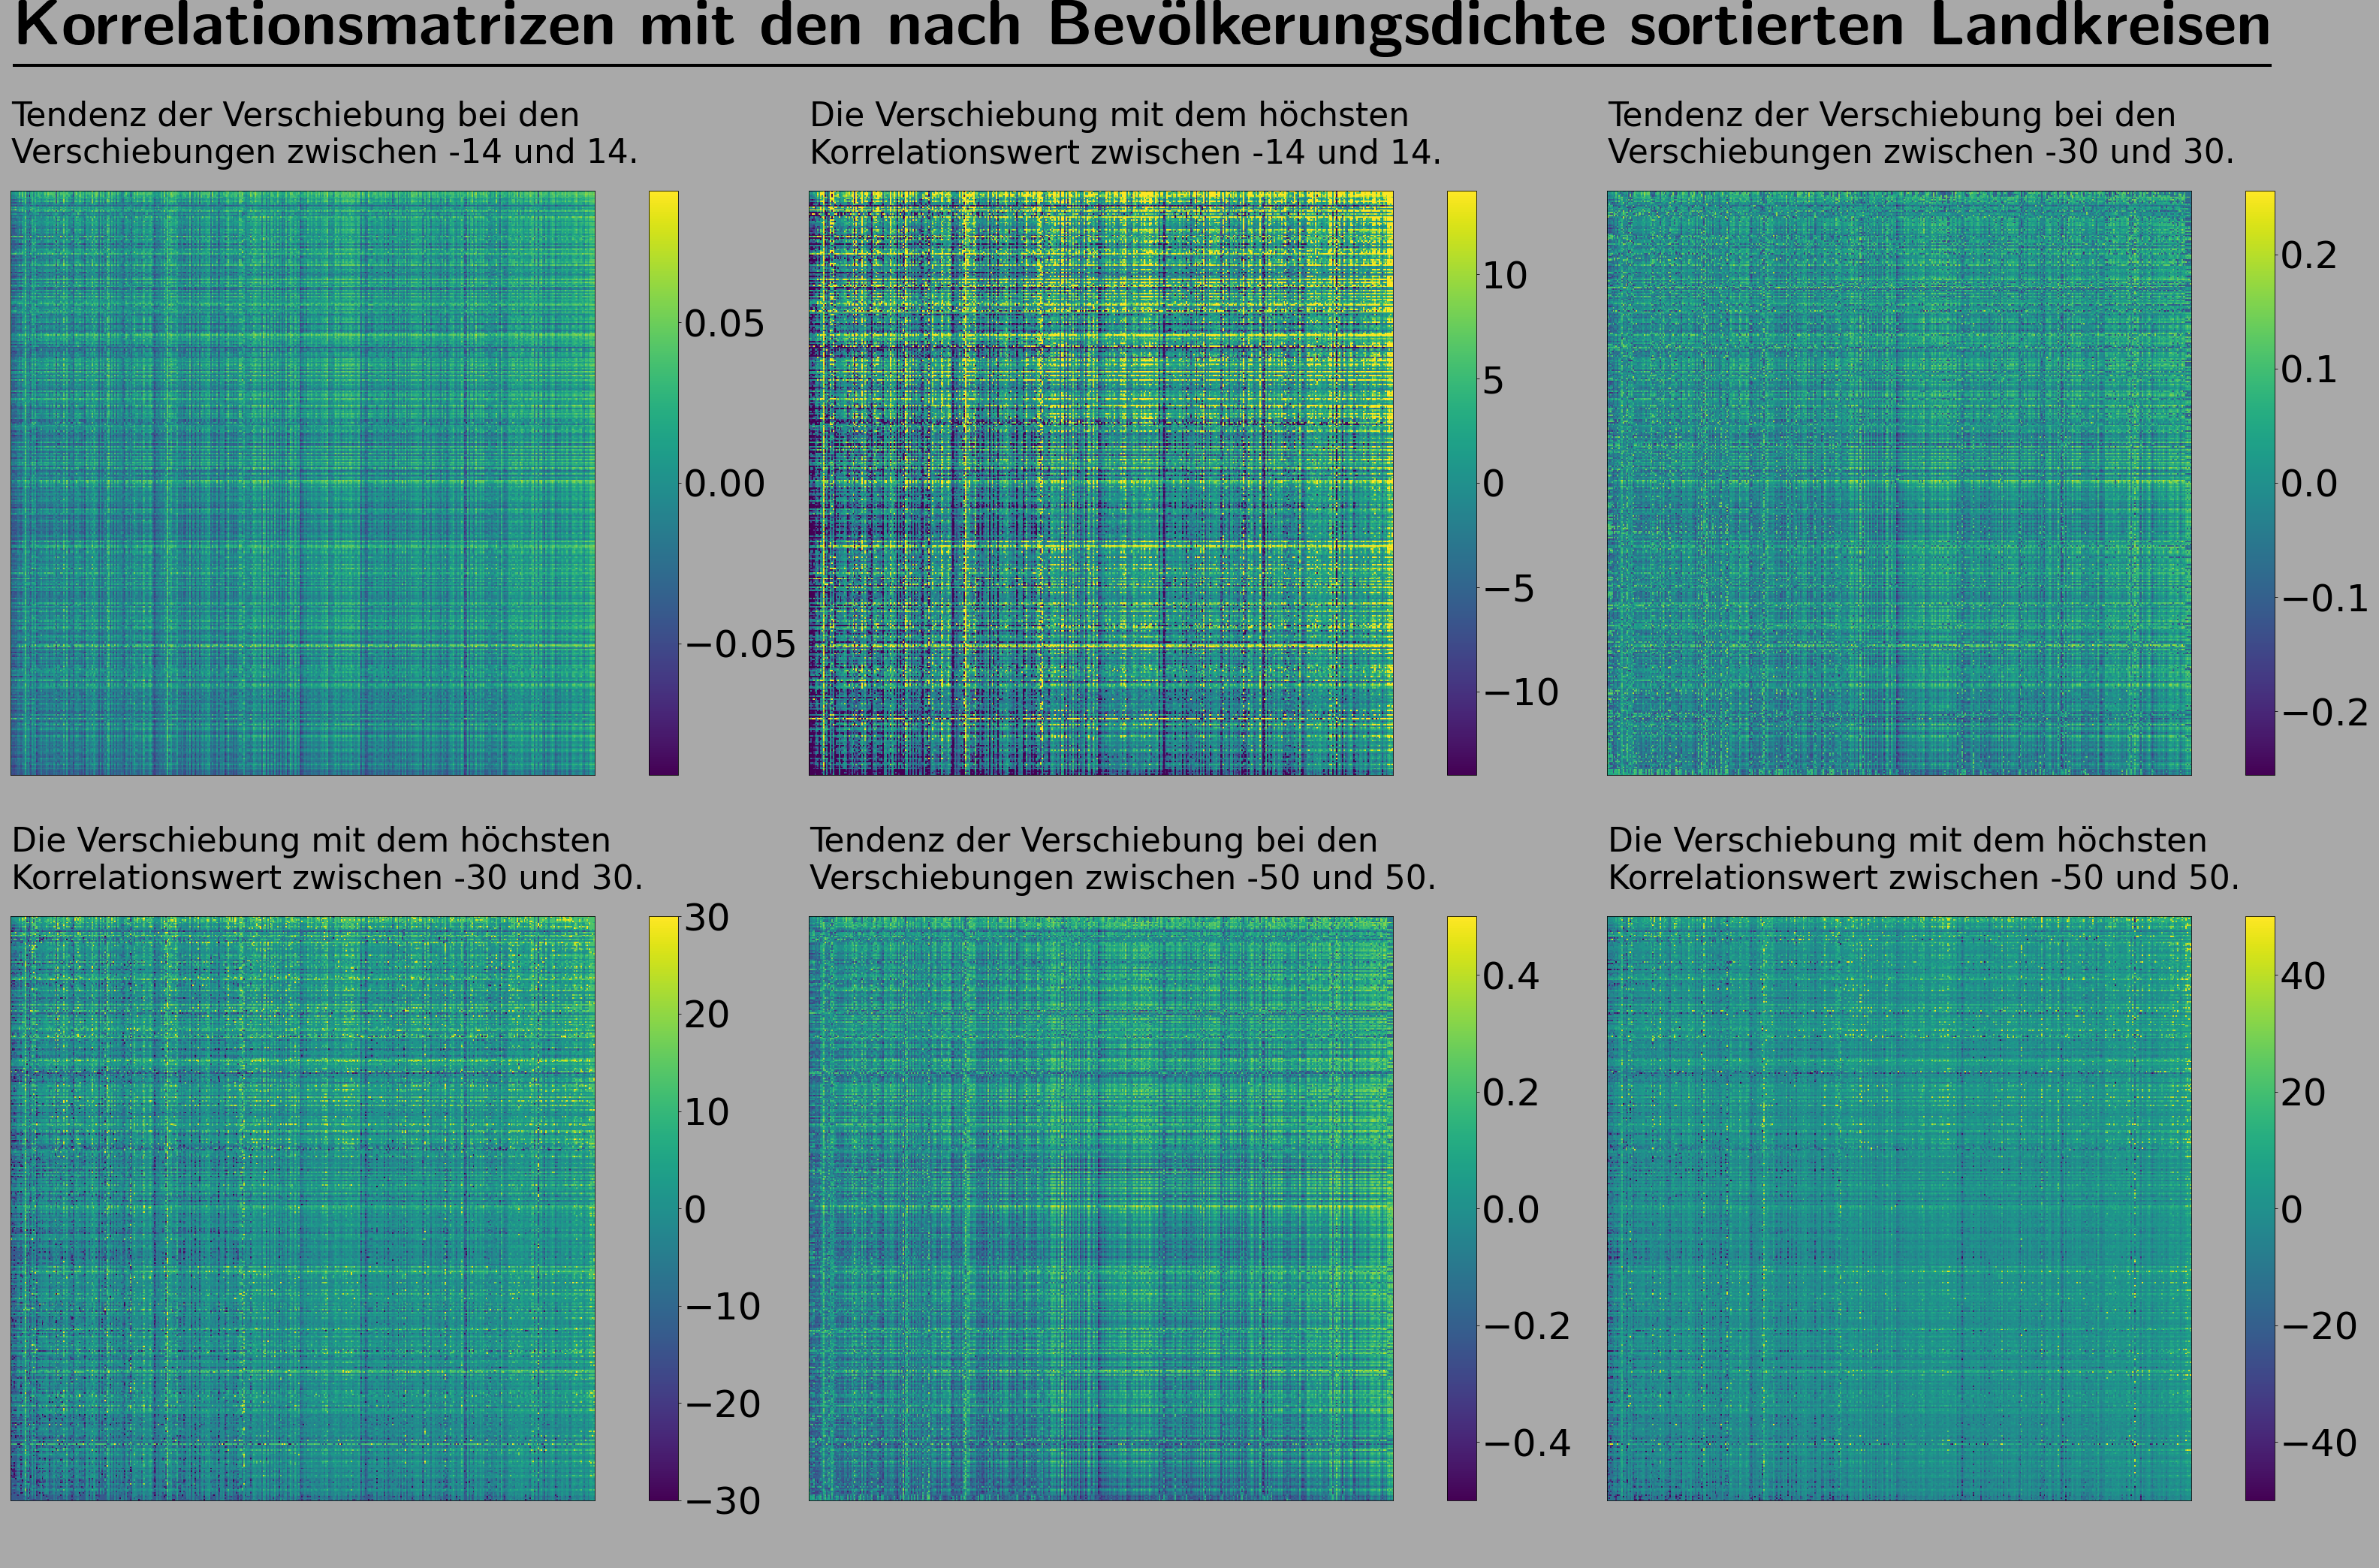
\includegraphics[width = 0.95\textwidth]{figures/Ergebnisse/matrizes_pop_density_counties.png}
    \caption{Korrelationsmatrizen der Korrelationen aller Landkreise nach Bevölkerungsdichte sortiert (siehe \autoref{tab:counties_by_pop_density}). Die Farben der Zellen der oberen Matrizen entsprechen den Tendenzen der Verschiebung $\hat{\tau}$ des Landkreises der Spalte in Relation zum Landkreis der Zeile nach \autoref{eq:Tendenz der Verschiebung}. 
    In den unteren Matrizen wird die Zelle entsprechend der Verschiebung $\tau_0$ der Zeitreihe des Landkreises der Spalte entgegen der Zeitreihe der Zeile mit dem höchsten Korrelationswert $c(\tau_0)$ eingefärbt. Links sind die Kennzahlen aus den Verschiebungen $\tau\in[-14,14]$ und rechts aus den Verschiebungen $\tau\in[-30,30]$ ausgewählt und berechnet worden.}
    \label{fig:matrizes_pop_density_counties}
\end{figure}
\subsection{Korrelationsmatrizen mit den nach Bevölkerungsdichten sortierten Regierungsbezirken}\label{sec:Durchführung:Korrelationsmatrizen mit den nach Bevölkerungsdichten sortierten Regierungsbezirken}
Die vier Matrizen mit den Werten für die Korrelationen zwischen den Regierungsbezirken finden sich in \autoref{fig:matrizes_pop_density_districts}. Die Matrizen sind gemäß \autoref{sec:BeschreibungKorrelationsanalyse} und \autoref{sec:Vorgehensweise:Korrelationsanalyse} erstellt. Die Zeilen und Spalten sind nach der Bevölkerungsdichte der Regierungsbezirke sortiert, die vollständige Auflistung befindet sich im Anhang in \autoref{tab:districts_by_pop_density}.

In den Matrizen in \autoref{fig:matrizes_pop_density_districts} ist die in \autoref{sec:Durchführung:Korrelationsmatrizen mit den nach Bevölkerungsdichten sortierten Landkreisen} beschriebene Verteilung der Werte von ansteigend von links nach rechts noch deutlicher zu erkennen. Auch die Ausnahmen, wie beispielsweise der Regierungsbezirk Trier, dem die vierte Spalte zugeordnet ist: Diese Spalte fällt durch erstaunlich hohe Werte auf, wohingegen die Werte links davon sehr einheitlich blau sind. Auch die beiden Spalten rechts davon enthalten relativ hohe Werte, jedoch nicht ganz so extrem wie die Spalte des Regierungsbezirks Trier.
\begin{figure}[H]
    \centering
    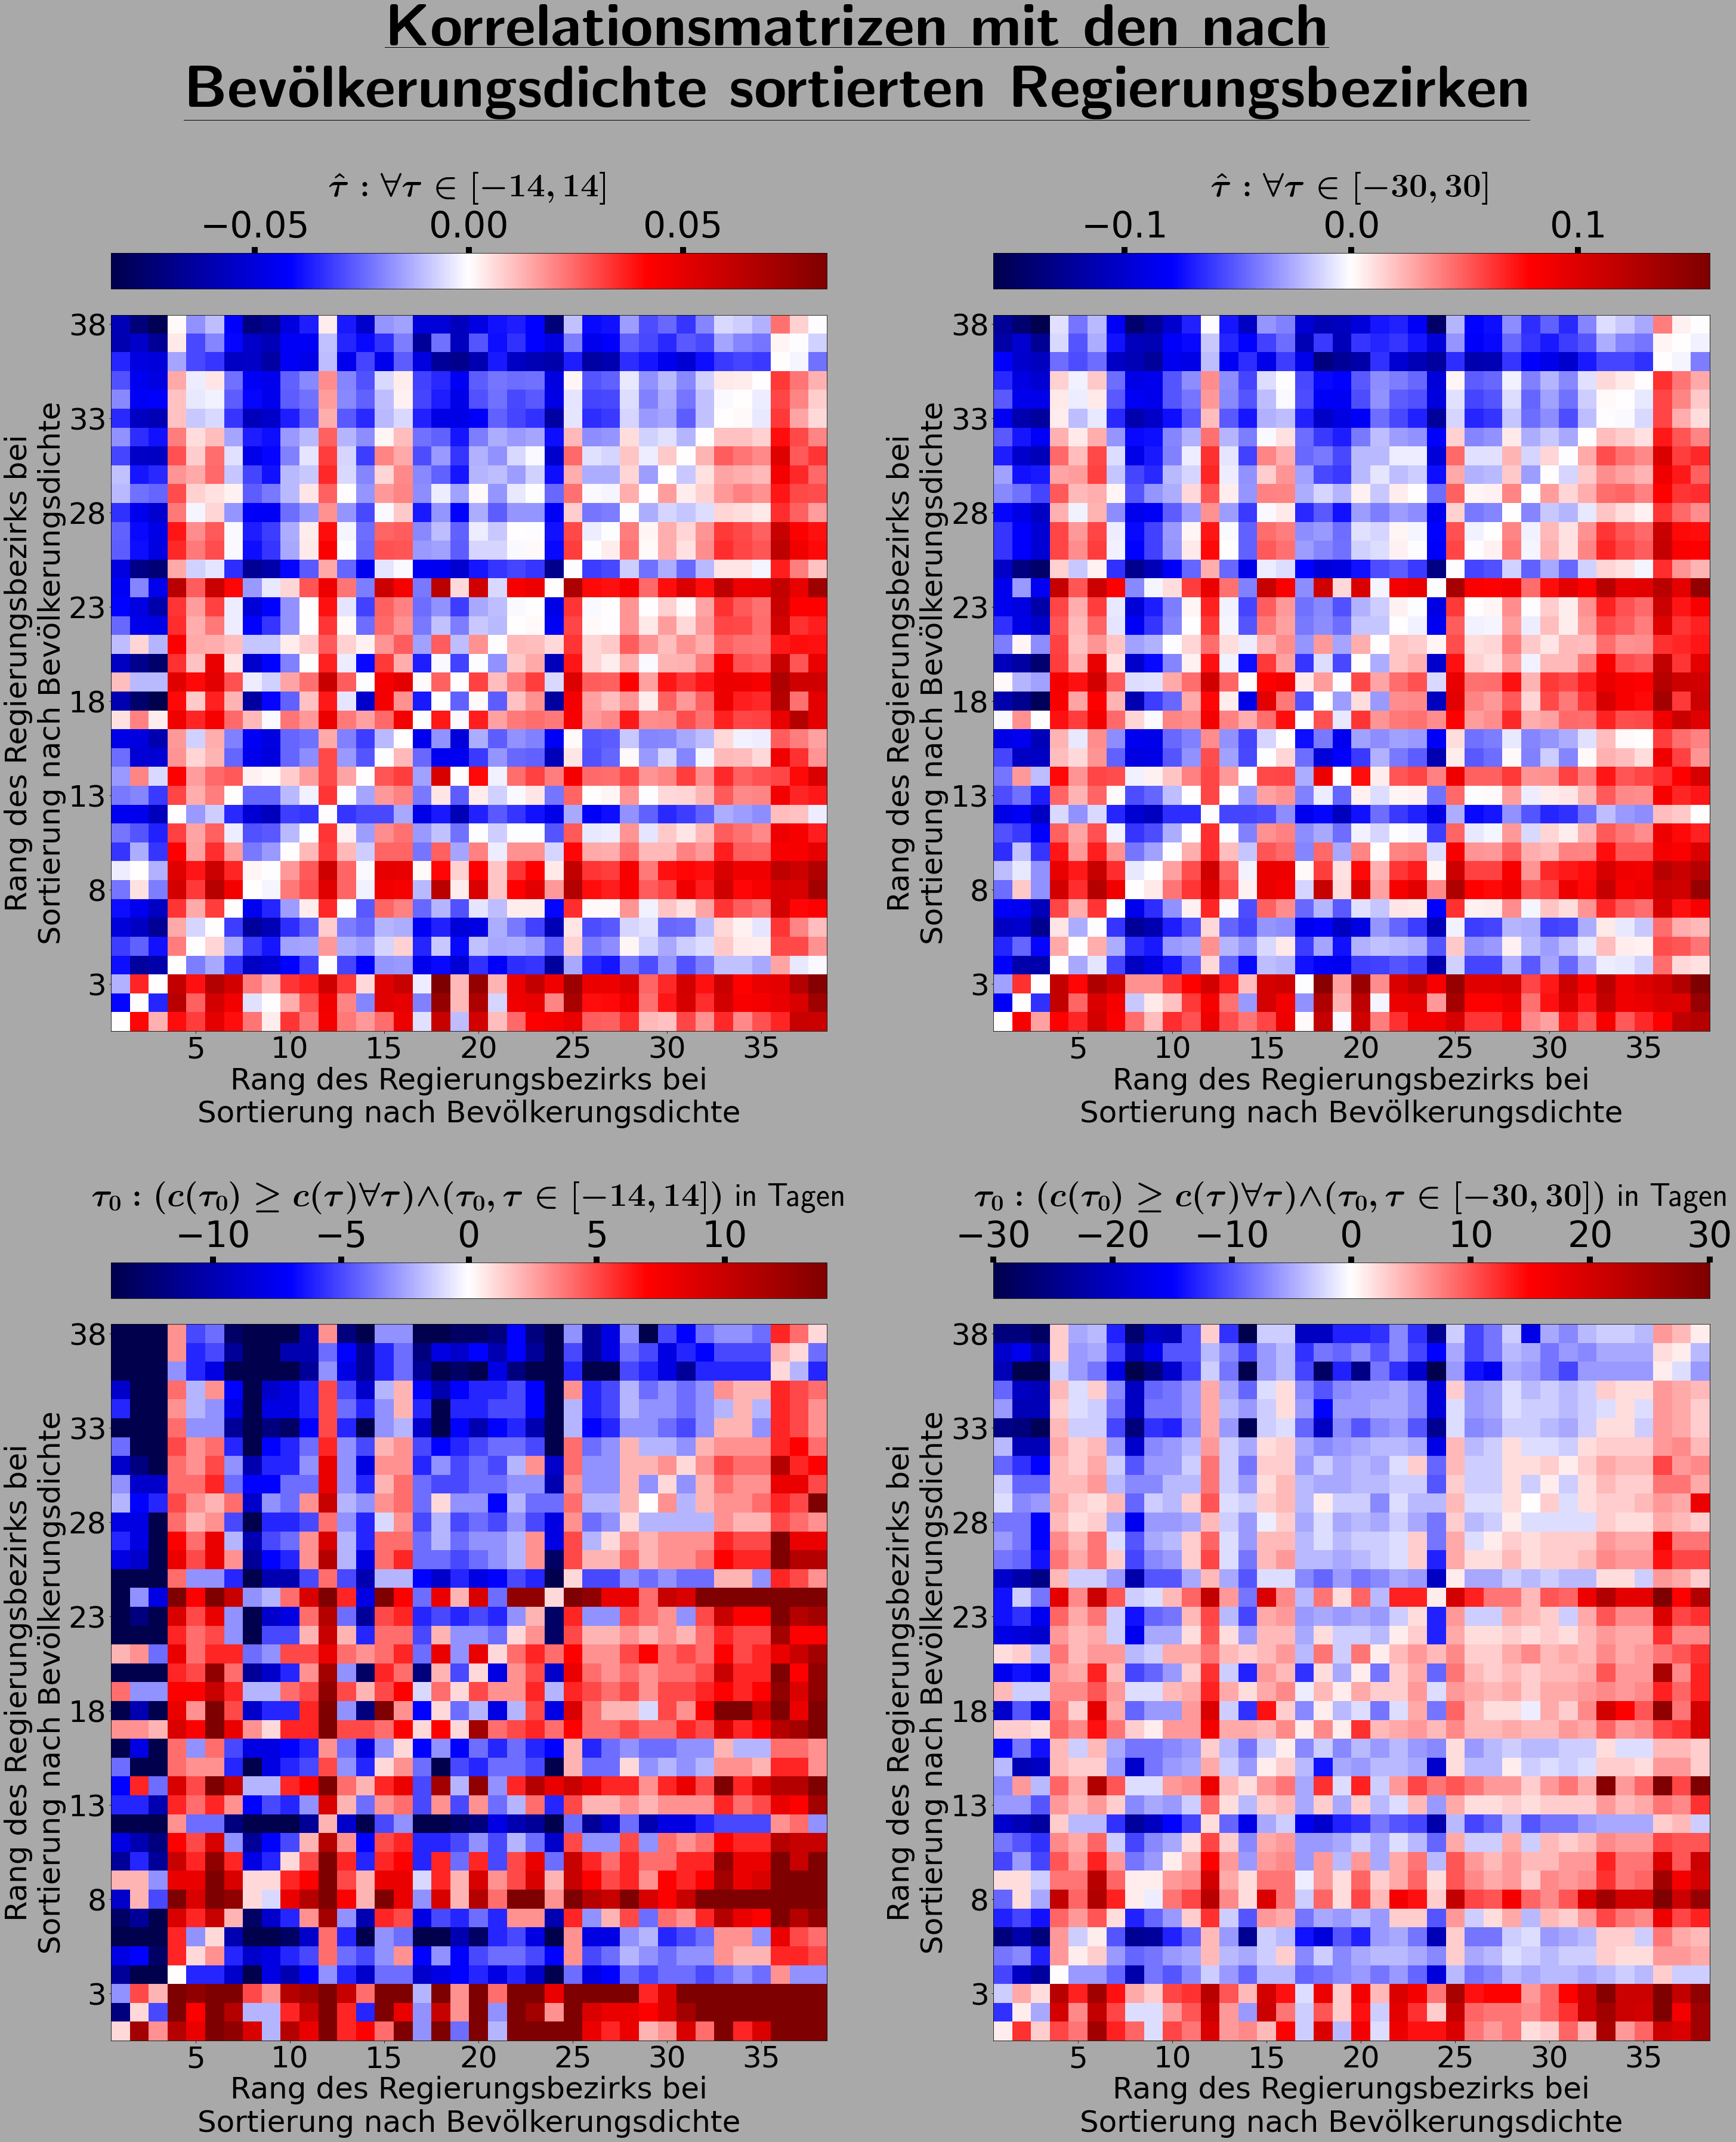
\includegraphics[width = 0.95\textwidth]{figures/Ergebnisse/matrizes_pop_density_districts.png}
    \caption{Korrelationsmatrizen der Korrelationen aller Regierungsbezirke nach Bevölkerungsdichte sortiert (siehe \autoref{tab:districts_by_pop_density}). Die Farben der Zellen der oberen Matrizen entsprechen den Tendenzen der Verschiebung $\hat{\tau}$ des Regierungsbezirks der Spalte in Relation zum Regierungsbezirk der Zeile nach \autoref{eq:Tendenz der Verschiebung}. 
    In den unteren Matrizen wird die Zelle entsprechend der Verschiebung $\tau_0$ der Zeitreihe des Regierungsbezirks der Spalte entgegen der Zeitreihe der Zeile mit dem höchsten Korrelationswert $c(\tau_0)$ eingefärbt. Rechts sind die Kennzahlen aus den Verschiebungen $\tau\in[-14,14]$ und rechts aus den Verschiebungen $\tau\in[-30,30]$ ausgewählt und berechnet worden.}
    \label{fig:matrizes_pop_density_districts}
\end{figure}

